

\chapter{Introduction}
Recently there has been great advances in wearable electronics. In parallel, there are rapid advances in machine learning~\cite{abadi2016tensorflow,silver2016mastering}, mainly driven by an increasing number of transistors, governed by Moore's law, which states that transistor count doubles every year. The graph~\ref{fig:Moores_law} demonstrates that computing, as driven by Moore's law, generally advances faster than the number of shipped MEMS sensors for wearable applications~\cite{nissila2014ihs}. Custom hardware is harder to scale than software, and it has large variations due to market demands, as shown on~\ref{fig:Moores_law}. 

To leverage the advantages of computing power, we need to find better ways to systematically collect data on our bodies.  As evident by the smartwatches domination of the wearable sensor market~\cite{allAboutWrist}, the current paradigm of wearable sensors affords us to collect data or actuate just from one location. Furthermore, they require manual manipulation and placement. Almost for all wearable sensors, the position plays a significant role. 

\begin{figure}[!ht]
\centering
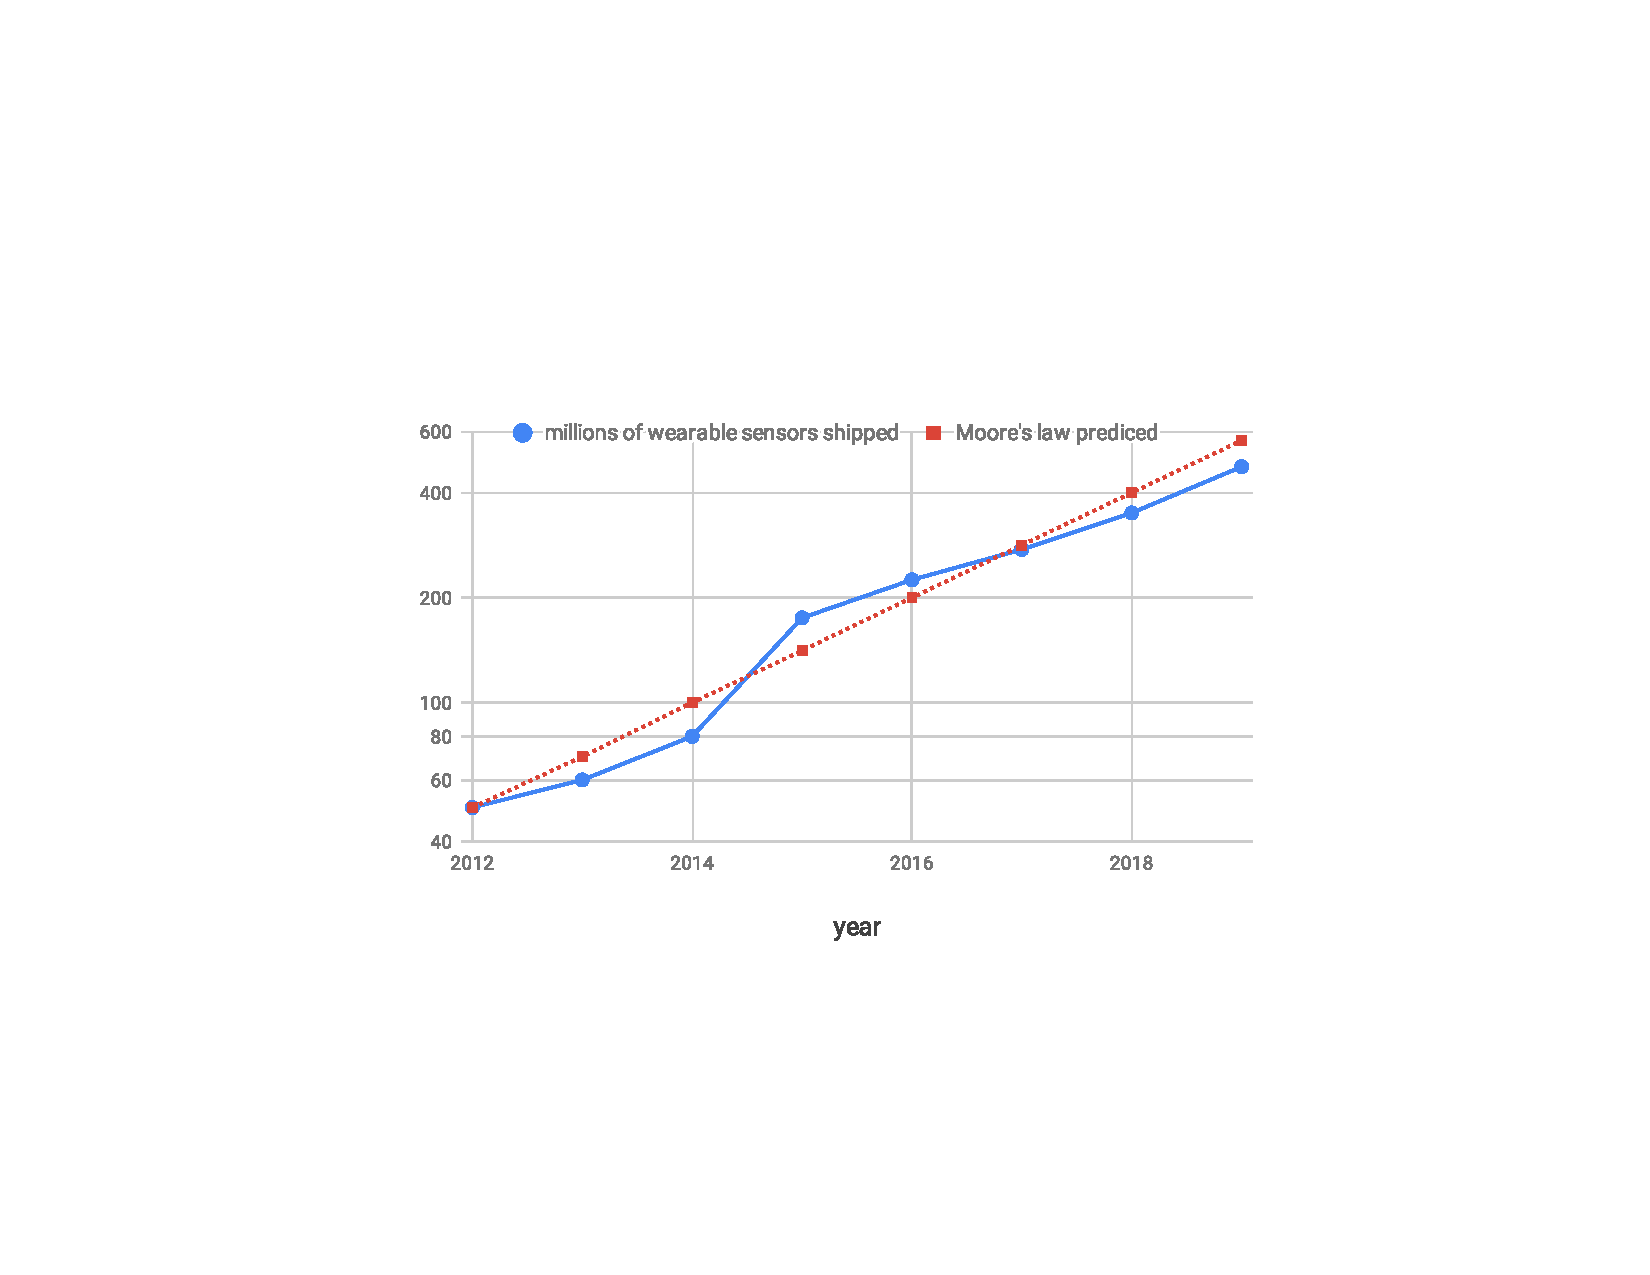
\includegraphics[width=\textwidth]{pictures/chapter1/Moor_law_graph.pdf}
\caption{Comparison between millions of shipped MEMs sensors for wearable devices vs predicted by Moore's law.}
\label{fig:Moores_law}
\end{figure}

This thesis proposes and explores wearable devices that move autonomously on the human body as mini robots. We named this idea Dynamic Wearable Technology (DWT).  Specifically, the thesis introduces two complementary robots: \textit{Epidermal robots} that can move on the skin, and \textit{Rovables} that move on the clothing. The specification of the robots are summarized in table~\ref{fig:Table_robots_specs}.

Robotics is a relatively new field, with first industrial robots appearing in the early 1960s~\cite{nof1999handbook}. As a result, there is not much crucial historical context. Miniature robots require sophisticated electronics with low power consumption and MEMS fabrication. Such robots have only become accessible in recent years, due to improvements in microfabrication. On the other hand, living creatures were used on the human body for a long time. For example, in Mexico and ancient Egypt, a beetle on a chain was used as jewelry~\cite{BettleJewelry}. Maggots are used for chronic diabetic ulcers~\cite{sherman2003maggot} and leeches have been used for medical purposes for more than 2500 years~\cite{singh2010medicinal}.

\begin{figure}[!ht]
\centering
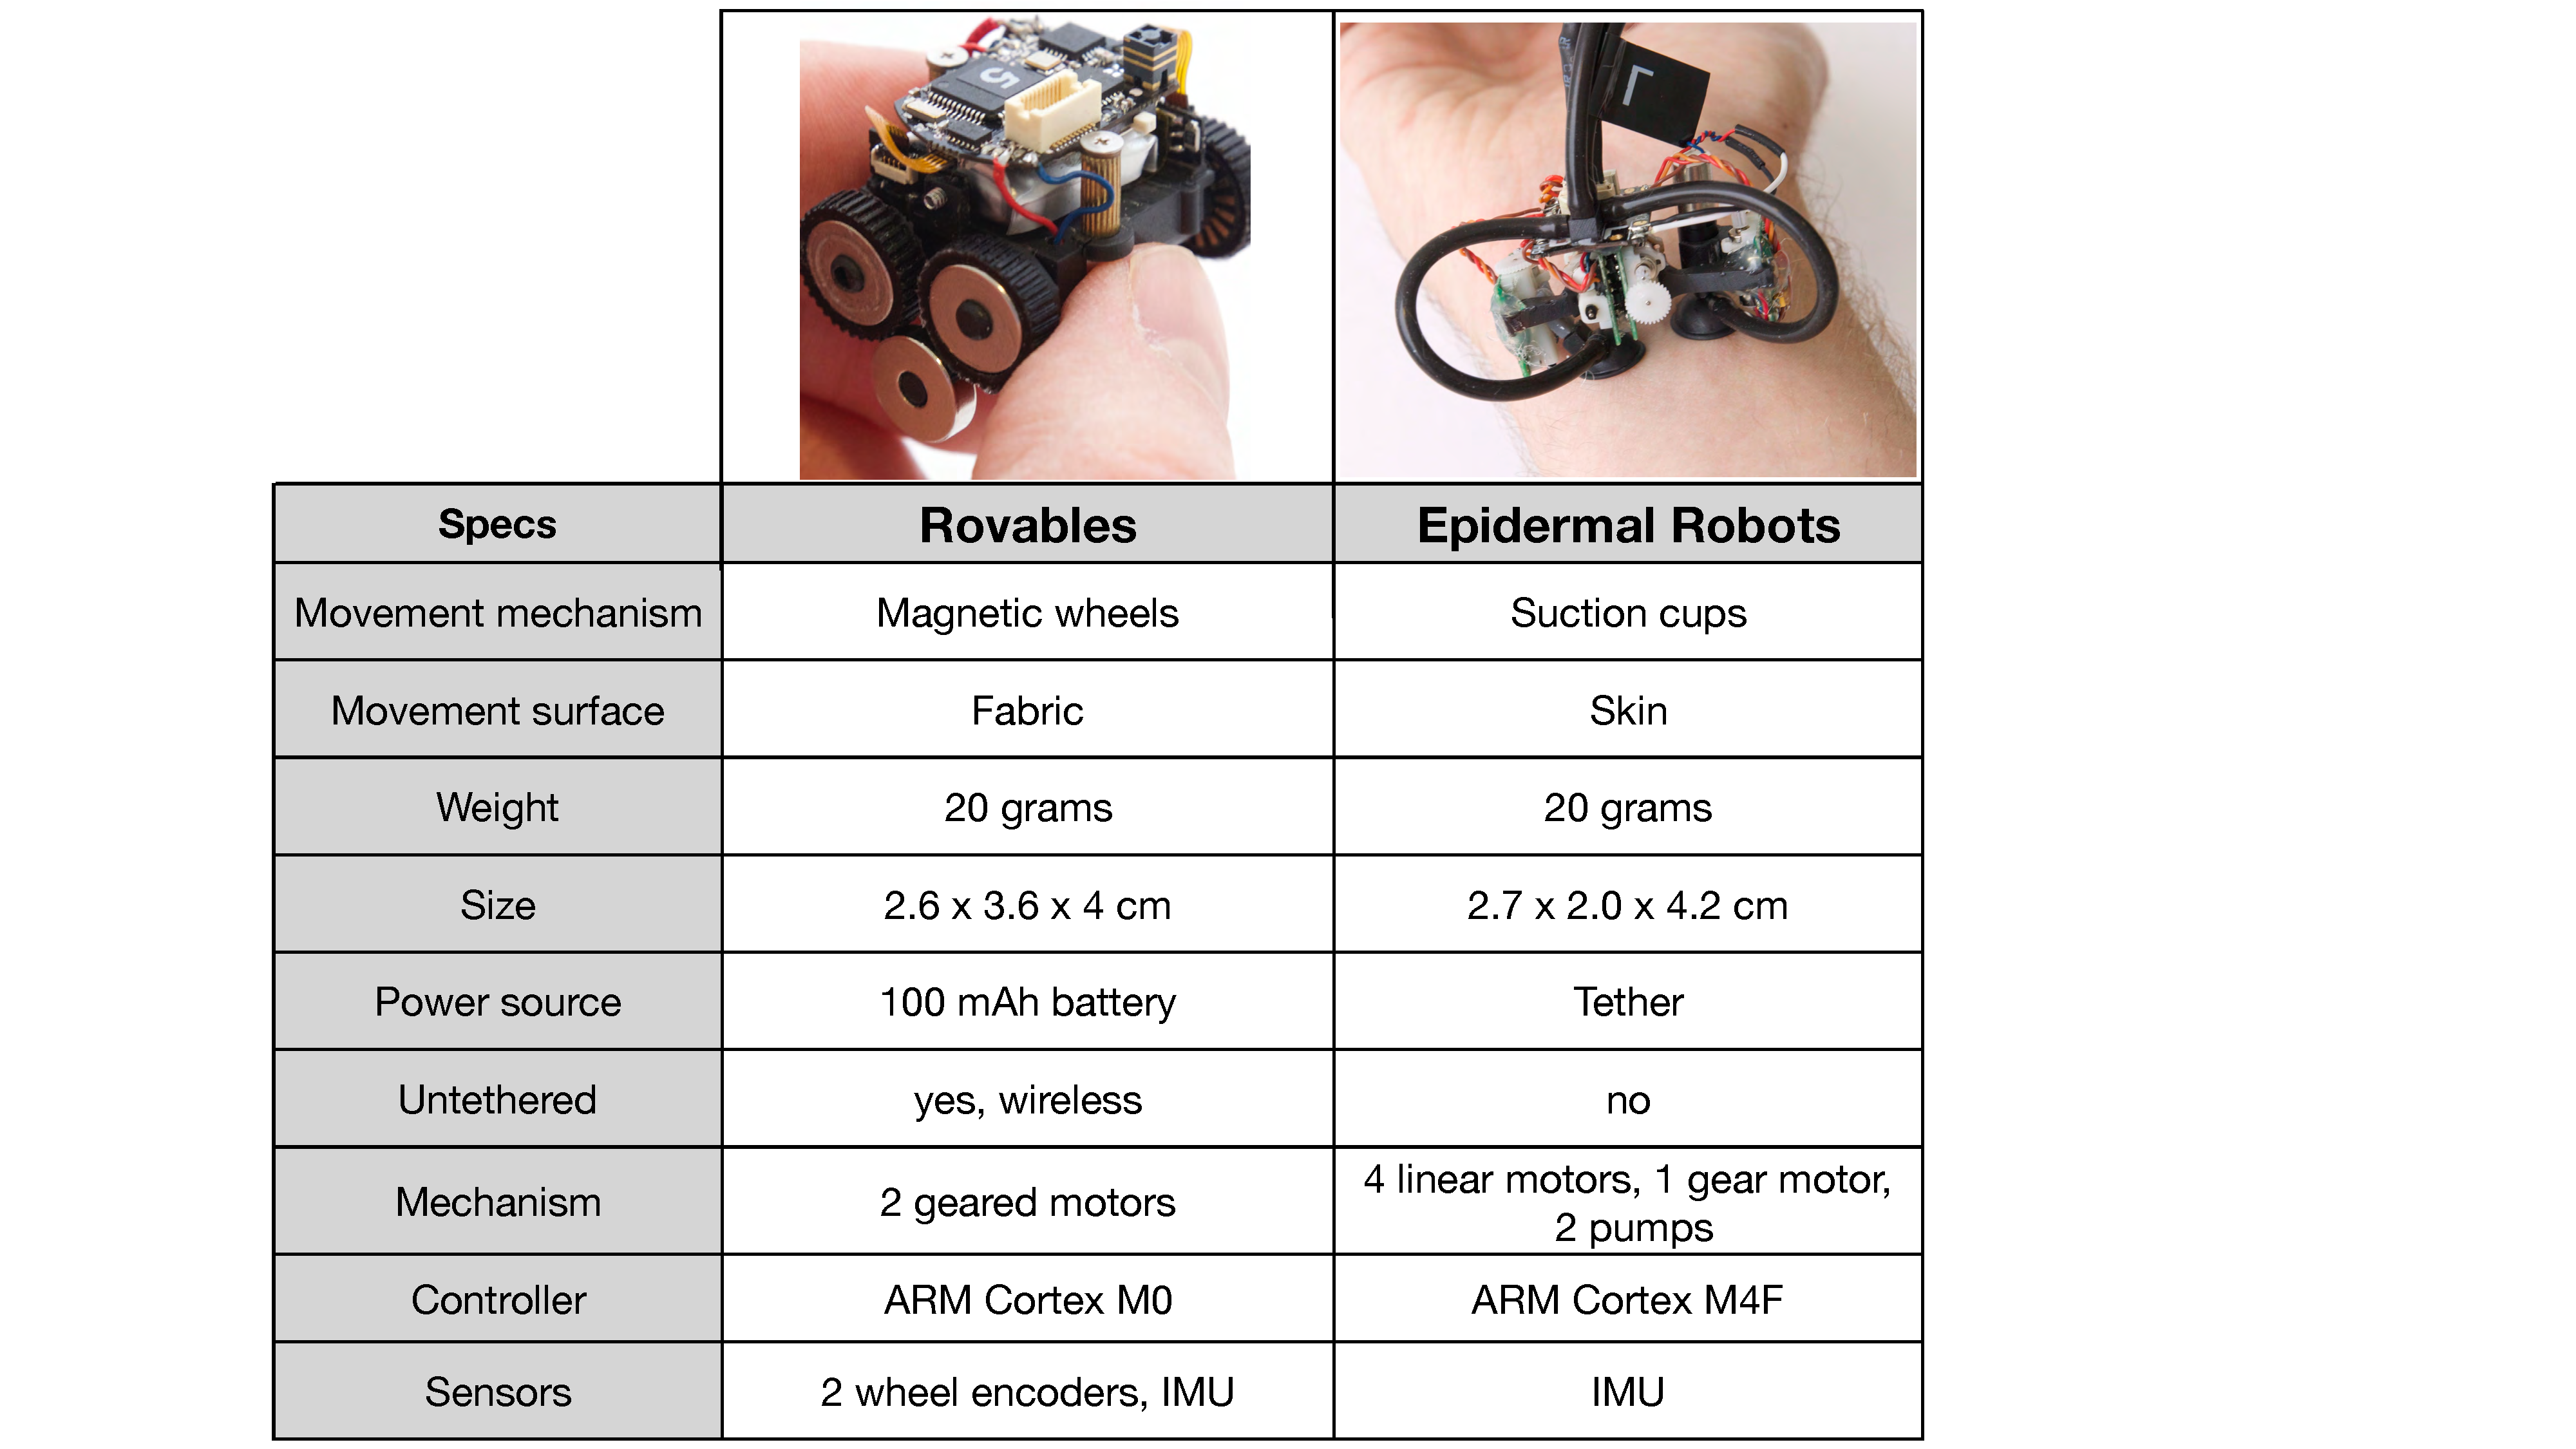
\includegraphics[width=\textwidth]{pictures/chapter1/table_two_robots.pdf}
\caption{Selected specification of the two designed robots. }
\label{fig:Table_robots_specs}
\end{figure}

\begin{figure}[!ht]
\centering
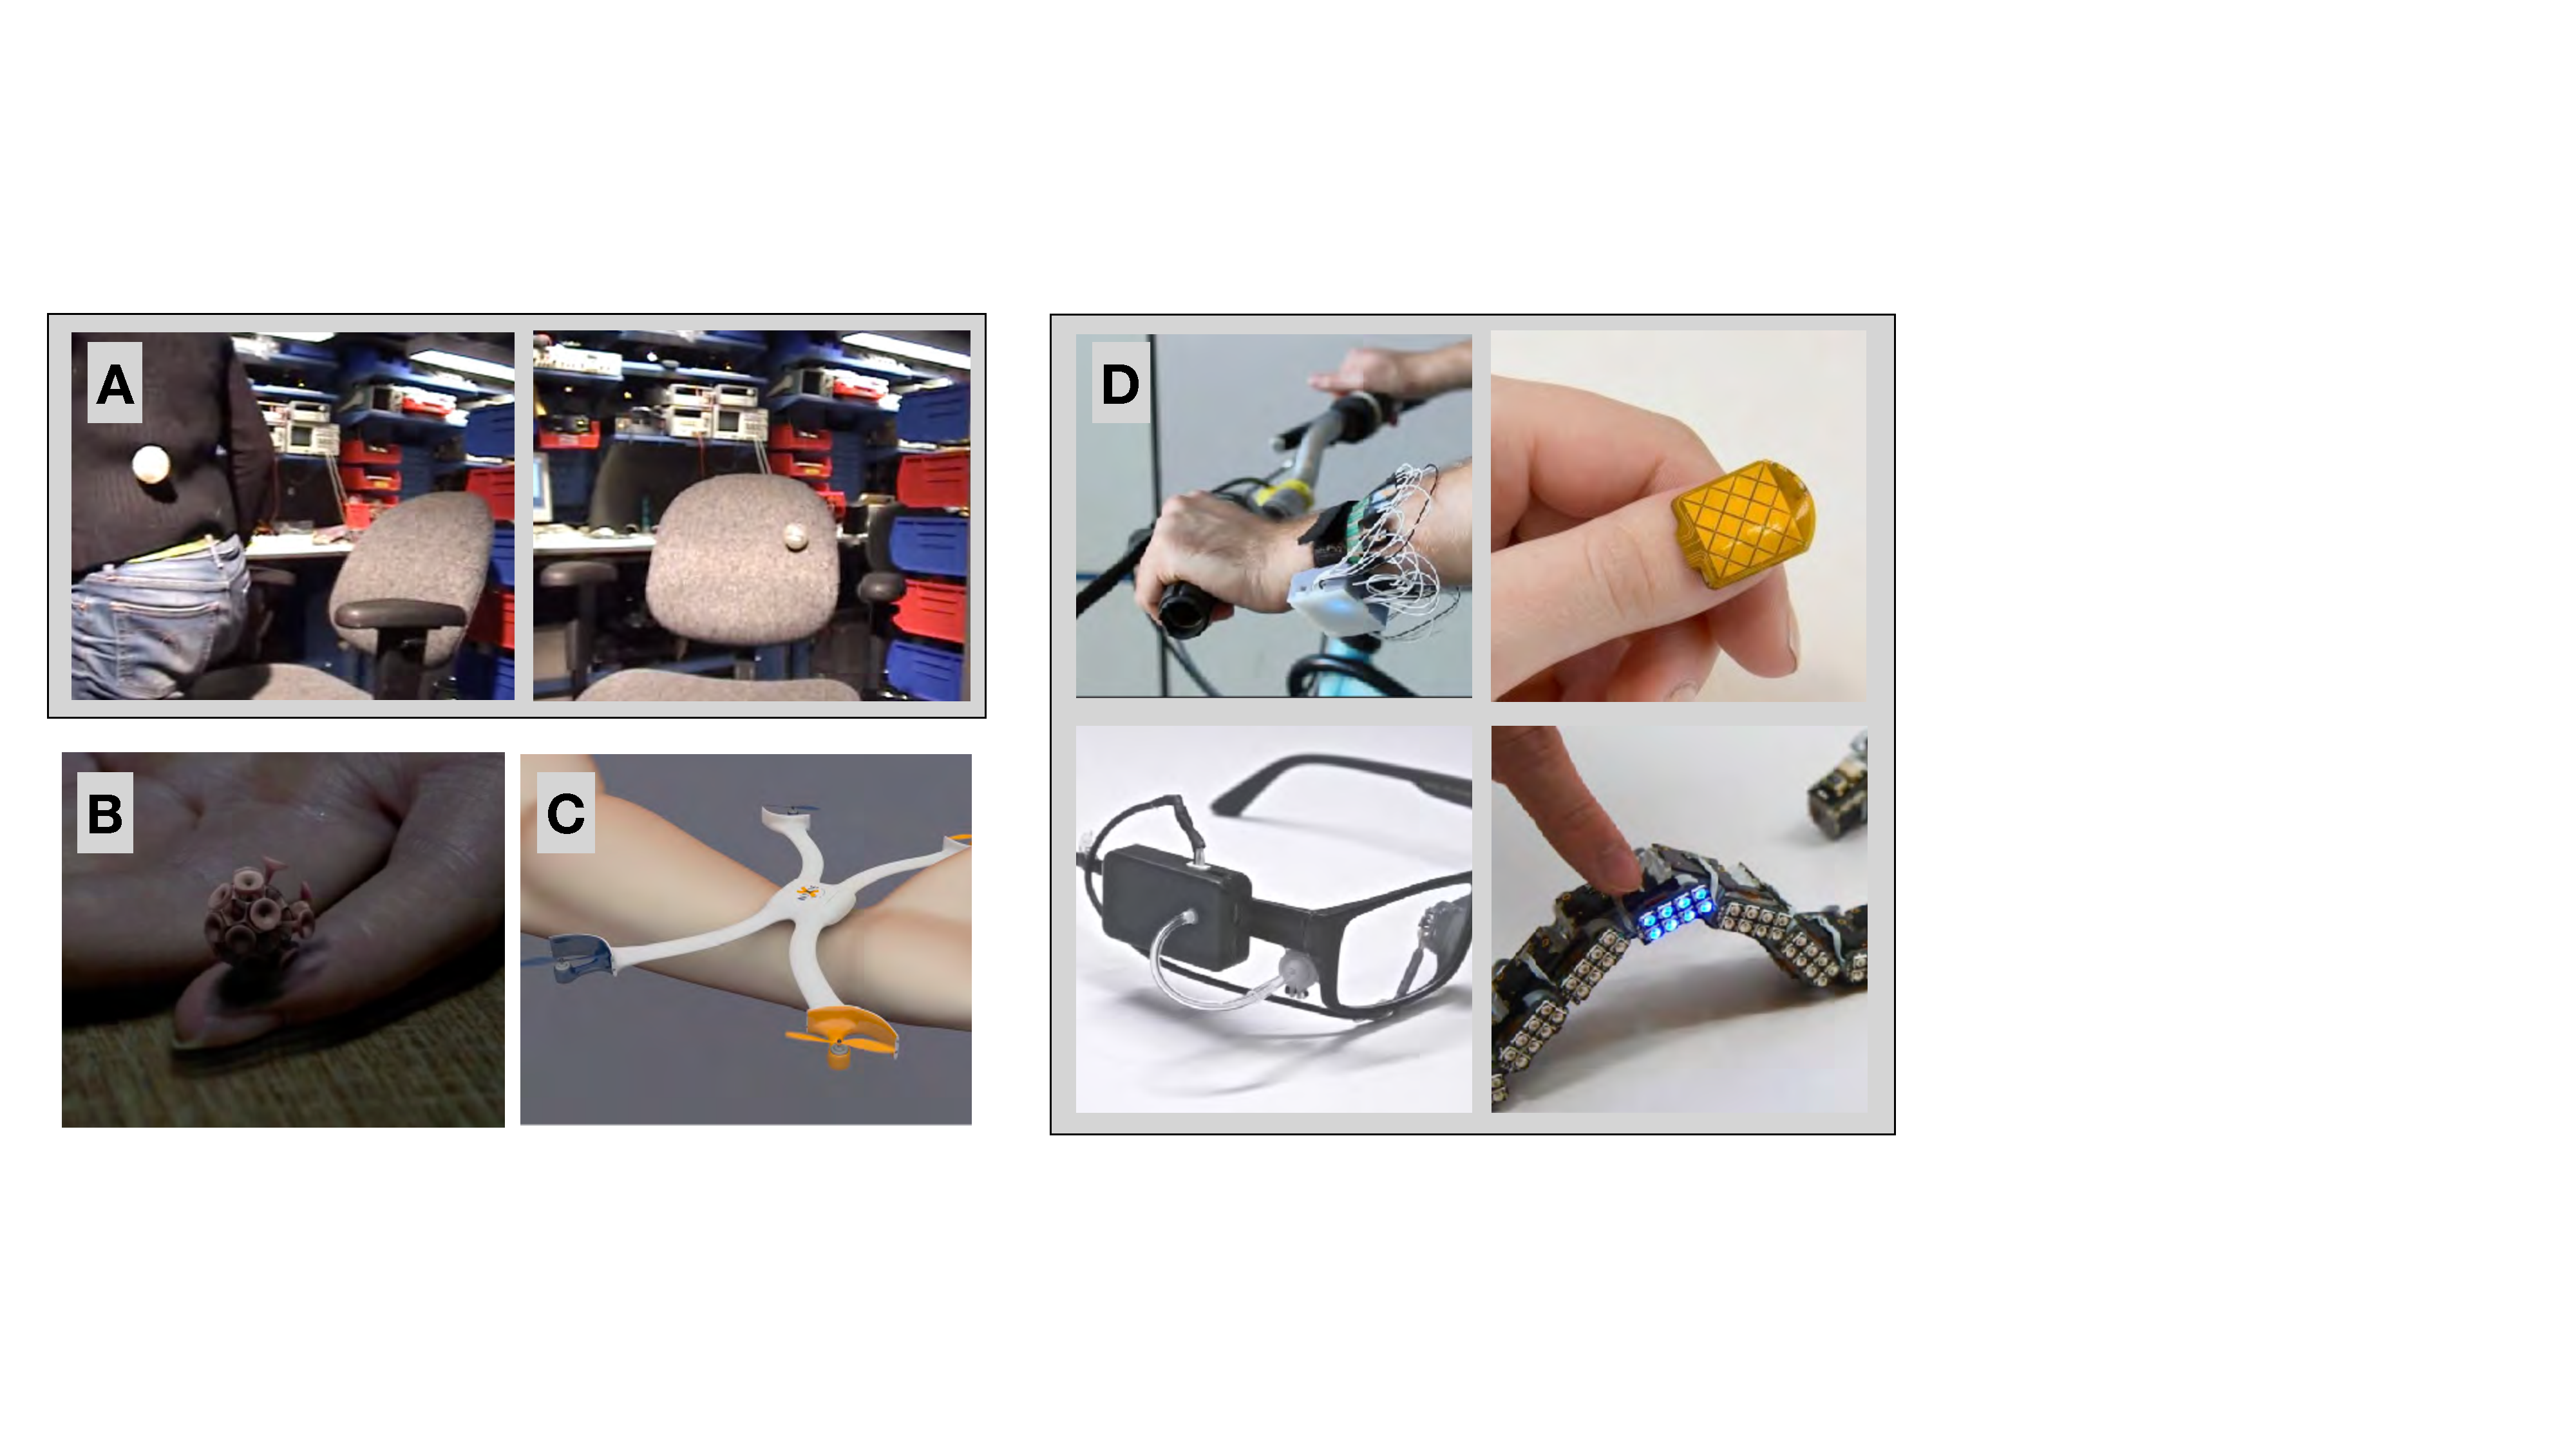
\includegraphics[width=\textwidth]{pictures/chapter1/inspirations.pdf}
\caption{Inspirations for DWT. A) Parasitic mobility. Robots attached to the person, than to the chair. B) SkinSucka from Studio XO. A concept video with skin crawling robots. C) Nixie, a drone thats also a bracelet. D) My previous research in wearables and robotics. }
\label{fig:inspirations}
\end{figure}

%inspirations
There are three inspirations for this work. First, Nixie bracelet drone~\cite{nixieDrone} from Intel's Make it Wearable competition, led me to believe that wearable technology does not need to be static.  Second, a concept of parasitic mobility~\cite{laibowitz2005parasitic} was developed in 2005 in our research group: Responsive Environments at the MIT Media Lab. This concept showed sensor nodes that can hitchhike on a person, and detach where they are needed. Third, the previous work I did in medical imaging~\cite{dementyev2017dualblink,dementyev2013temperature} , wearables~\cite{dementyev2014wristflex,kao2015nailo} and robotics~\cite{nakagaki2016chainform,dementyev2016rovables}. Doing those projects allowed me to understand the limitations of the current technologies and build up the technical skill required for this thesis. Those three ideas lead to the Rovables project. Later, I saw a concept video~\cite{SkinSucka} from a design firm Studio XO. In the video, small robots moved around the body and applied makeup, which I found to be intriguing. This video, together with my interest in medical applications led to the development of the SkinBot robot and the area of epidermal robots.

The small climbing robots could be used for other purposes then wearable devices. For example, they could be used for finding cracks in an airplane engine or climb mountains. This type of robots has been explored in robotics field in great detail before~\cite{lam2011flexible,eich2011design}. This thesis examines only wearable applications to avoid broad but shallow exploration of this topic.  Also, I believe that the blend of wearable electronics and robotics is a new area of research. 

% What is DWT
\section{Dynamic wearable technology (DWT)}
In this section, we attempt to outline the main design criteria of DWT robots. Each of those criteria is discussed in separate chapters in the thesis. To satisfy those criteria, the system design of the DWT robot needs certain subsystems. In Figure~\ref{fig:overall_system} we provide a block diagram of a DWT robot.
\begin{itemize}
    
\item \textbf{Small size (Chapter 4)}. \textit{}The robots should be at least an order of magnitude smaller than the human body, millimeters to few centimeters in size. First, small robots are less obtrusive to the human host. Second, it is easier for a small robot to move around a complex surface such as the human body. Generally, the human body can be thought of as cylindrical.  surfaces~\cite{dodig2016models}. To a robot that is an order of magnitude smaller, such surfaces will appear flat. 
\item \textbf{Ability to move freely (Chapter 5)}. The robots should have the ability to move freely on human clothing or skin. They should be able to move vertically as well.
\item \textbf{Autonomous (Chapter 5,~8)}. The robots should be able to navigate the human body on their own. Navigation requires a localization method and a map.  The robot operation should not require any external sensors or devices. 
\item \textbf{Platform (Chapter 6)}. DWT should be able to support different types of sensors or actuators, so different applications can be developed. 
\end{itemize}

\begin{figure}[!ht]
\centering
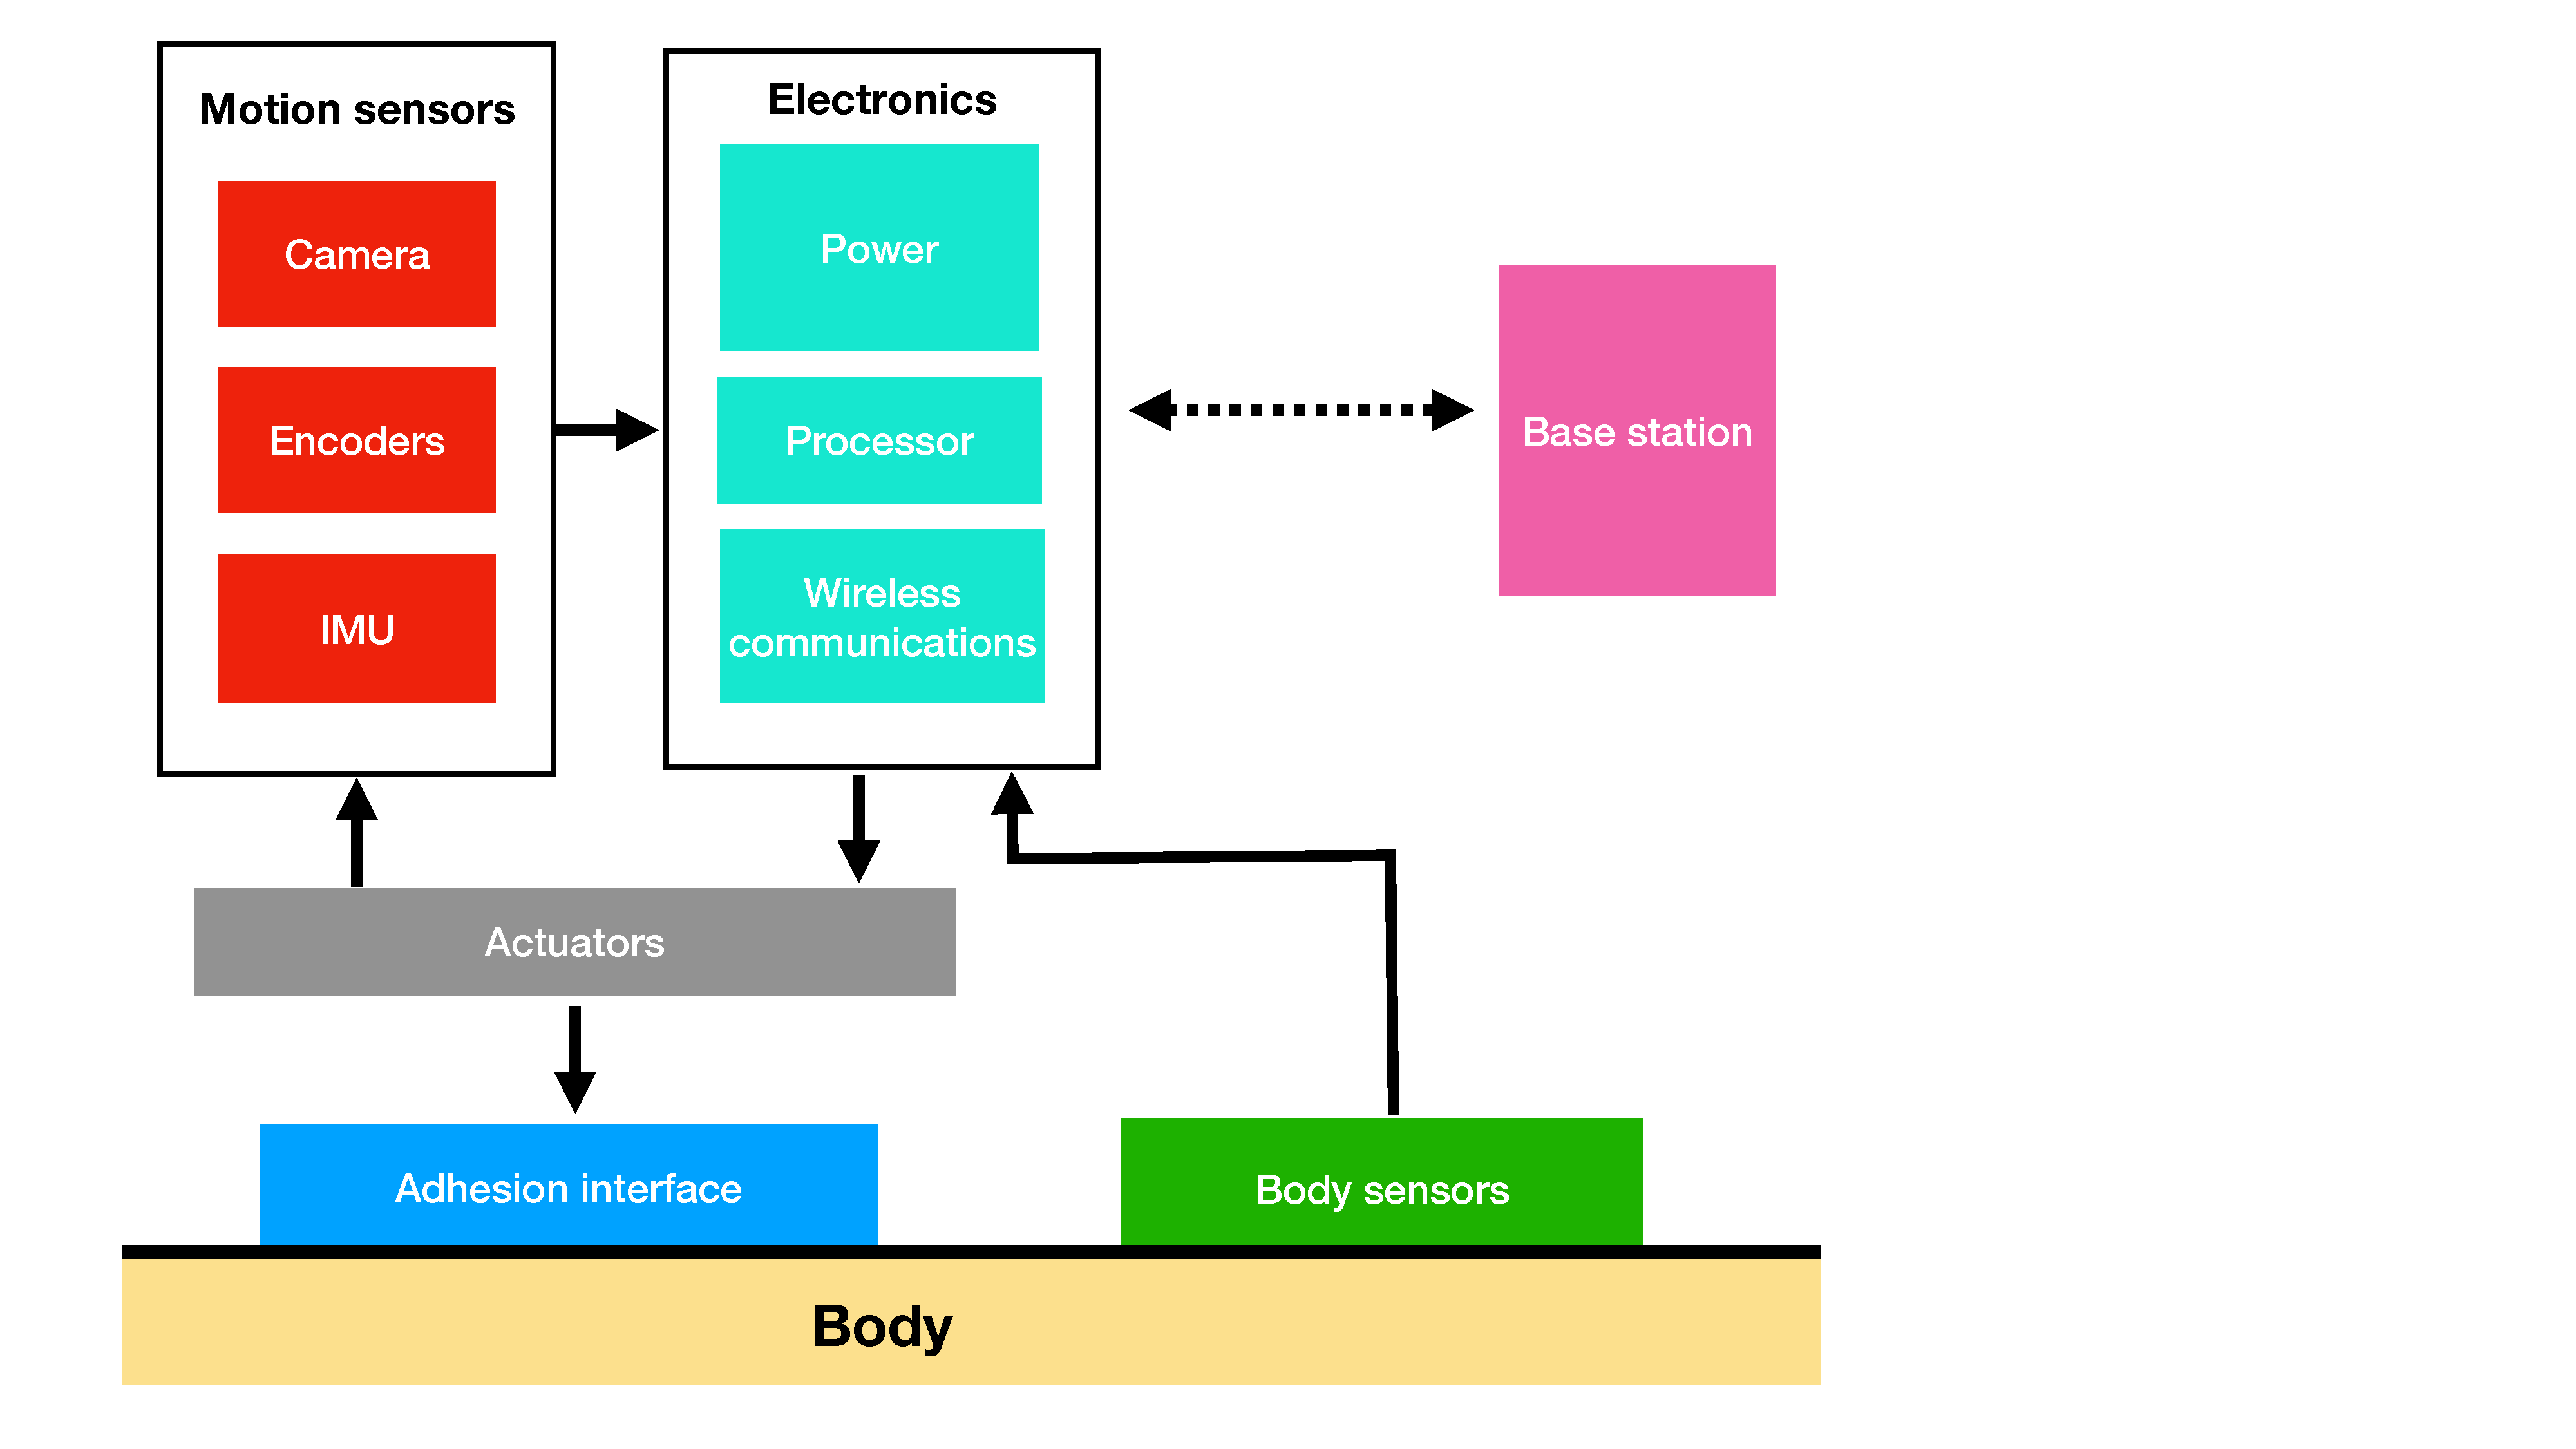
\includegraphics[width=\textwidth]{pictures/chapter1/robots_systems.pdf}
\caption{The overall system diagram of DWT robots. The arrows show the infromation flow between the subsystems. }
\label{fig:overall_system}
\end{figure}

\section{Why is DWT important}
Let's imagine a future scenario where we already have small robots that fulfill the previous requirements. Medicine is becoming more personalized and data-driven and will continue to do so in the future~\cite{piwek2016rise}. Potentially, DWT will become our first line of defense against diseases. To do a yearly medical check, instead of going to a doctor or a hospital, one would order online a personalized box of robots,  tailored for a specific purpose. After receiving the robots, the person would put the robots on, perhaps while going on through everyday routine or sleeping during the night. The robots will take repeatable and high-resolution measurements of the body. The robots could see things that are impossible for a doctor to see with a naked eye. For example, robots can test the mechanical properties of the skin to detect very early signs of cancers. All the data is collected and analyzed with powerful computers remotely.  If the robots discover something, they could use a precise laser to remove the problematic skin cells. Also, the robots can see invisible signals of the body, such as bioelectrical potentials (EKG and EMG). Once the robots finish, they can be shipped back, just like returns with online shopping. 

DWT can be used in many fields, such as medical sensors, human-computer interactions, body-care, arts, and fashion. I will provide specific example applications throughout the thesis. Currently, I believe the most productive use is medical sensing, as it can have an immediate improvement in our lives. Chapter 2 (Background) provides a  thorough comparison to other technologies. Below, I will attempt to summarize the benefits of DWT. 
All DWT posses the following characteristics.
\begin{itemize} 
\item \textbf{Continous and repeatable measurements}. The robots eliminate errors and uncertainties associated with human operators. 
\item \textbf{Full-body coverage}. The robots can access any location on the body. 
\item \textbf{Easy to transport}
The small and lightweight robots are easy to transport to a remote location or home. It is a great benefit for individuals with limited mobility or in remote locations with no access to sophisticated instruments. 
\end{itemize} 


Depending on the applications, the robots might posses additional benefits: 
\begin{itemize} 

\item \textbf{Ability to work in swarm}. The robots could work together to coordinate tasks to accomplish them faster or to create sensor arrays. For example, one robot could serve as a transmitter and other as a receiver. 
\item \textbf{Sophisticated sensors and actuators}. The robots are not limited to simple sensors, as many current wearables. As a payload, the robots can carry sophisticated sensors, such as cameras. 
\end{itemize}

\section{Chapter and thesis summaries}
The thesis has four main parts: First part (\textbf{chapter 1,2}) provides an overview of DWT, as well as describes previous work and technologies. A second part (\textbf{chapter 3,4}) dives deep into the implementation of Epidermal robots and Rovables. This part is primarily based on my previously published work on this topic~\cite{dementyev2016rovables,dementyev2018epidermal,kao2017exploring,dementyev2017skinbot}. The third part (\textbf{chapter 5,6,7,8}) provides a discussion of the main design criteria of DWT, such as power consumption, navigation, climbing, and size. The fourth part (\textbf{chapter 9,10,11}) discusses applications of DWT, as well as limitations, future work, and concluding remarks.

%%------CONTRIBUTIONS---------------------
\section{Contributions of the thesis}
This thesis makes the following contribution:
\begin{enumerate}
\item We introduce a new area of \textit{Dynamic Wearable Technology}. 
\item As two instances of DWT, we develop Epidermal robots and Rovables. Epidermal robots can move on the surface of the skin. Rovables can move on the clothing.  All the design files and instructions are open-sourced online on Github\footnote{https://github.com/adementyev}
\item We discuss and study various points of DWT such as power consumption, size, and localization. 
\item We showcase various applications of DWT in medical, human-computer interactions and art domains. 
\end{enumerate}








